
\chapter{Schewe}
\label{chap:schewe}

\section{Theory}

This section is based heavily on \cite{Schewe2010} and partially adapts their results from B\"uchi to parity automata.

\begin{defn}
		Let $\mathcal{A} = (Q, \Sigma, \delta, c)$ be a DPA and let $\emptyset \neq C \subseteq M \subseteq Q$. Let $\mathcal{A}' = (Q', \Sigma, \delta', c')$ be another DPA. We call $\mathcal{A}'$ a \emph{Schewe merge of $\mathcal{A}$ w.r.t. $M$ by candidates $C$} if it satisfies the following:
	\begin{itemize}
		\item There is a state $r_M \in C$ such that $Q' = (Q \setminus M) \cup \{r_M\}$.
		\item $c' = c\upharpoonright_{Q'}$.
		\item Let $p \in Q'$ and $\delta(p, a) = q$. If $q \in M$ or if ($q \in C$ and $p$ is not reachable from $q$), then $\delta'(p, a) = r_M$. Otherwise, $\delta'(p, a) = q$. 
	\end{itemize}
\end{defn}

The definition of a Schewe merge is almost identical to that of a representative merge. The only difference lies therein that some additional transitions are redirected to the representative: when a transition leads to a candidate that is not in $M$ while also moving to a different SCC.

Using the Schewe merge instead of the representative merge does not actually remove any additional states from the automaton, it only provides a better \enquote{framework} for following algorithms such as the Moore reduction. Example figure \ref{fig:schewe:example_useful1} shows that using a Schewe merge followed by another merge of $\mu_M$ creates a better end result.

The automaton has six states. Regarding Moore equivalence, every state builds a singleton class. For priority almost equivalence, the classes are $\{q_0, q_1\}$, $\{q_2, q_4\}$, and $\{q_3\}$. As all states within one equivalence class lie in the same SCC, a representative merge w.r.t. $\mu_\text{skip}^{\equiv_\text{\Ankh}}$ will not change the number of states. However, a Schewe merge w.r.t. $\mu_\text{skip}^{\equiv_\text{\Ankh}}$ can result in figure \ref{fig:schewe:example_useful2}. Now, $q_0$ and $q_1$ are actually Moore equivalent and could be merged with $\mu_M$.

\begin{figure}
\centering
\begin{tikzpicture}[shorten >=1pt,node distance=2cm,on grid,initial text=]
  \node[state]           (0)                {$q_0,1$};
  \node[state]           (1) [right=of 0]   {$q_1,1$};
  \node[state]           (2) [above=of 0]   {$q_2,1$};
  \node[state]           (3) [right=of 2]   {$q_3,1$};
  \node[state]           (4) [right=of 3]   {$q_4,0$};
  \path[->] (0) edge [bend left] node [above] {a} (1)
  			(0) edge node [left] {b} (2)
            (1) edge [bend left] node [below] {a} (0)
            (1) edge node [below] {b} (4)
            (2) edge [bend left] node [above] {a,b} (3)
            (3) edge [bend left] node [below] {a} (2)
            (3) edge [bend left] node [above] {b} (4)
            (4) edge [bend left] node [below] {a,b} (3);
\end{tikzpicture}
\caption{Example to show the effect of a Schewe merge.}
\label{fig:schewe:example_useful1}
\end{figure}

\begin{figure}
\centering
\begin{tikzpicture}[shorten >=1pt,node distance=2cm,on grid,initial text=]
  \node[state]           (0)                {$q_0,1$};
  \node[state]           (1) [right=of 0]   {$q_1,1$};
  \node[state]           (2) [above=of 0]   {$q_2,1$};
  \node[state]           (3) [right=of 2]   {$q_3,1$};
  \node[state]           (4) [right=of 3]   {$q_4,0$};
  \path[->] (0) edge [bend left] node [above] {a} (1)
  			(0) edge node [left] {b} (2)
            (1) edge [bend left] node [below] {a} (0)
            (1) edge node [right] {b} (2)
            (2) edge [bend left] node [above] {a,b} (3)
            (3) edge [bend left] node [below] {a} (2)
            (3) edge [bend left] node [above] {b} (4)
            (4) edge [bend left] node [below] {a,b} (3);
\end{tikzpicture}
\caption{Automaton from figure \ref{fig:schewe:example_useful1} after Schewe merge.}
\label{fig:schewe:example_useful2}
\end{figure}

\begin{defn}
	Let $\mathcal{A}$ be DPA with a merger function $\mu : D \rightarrow 2^Q$. For a representative merge $\mathcal{A}'$, we define the \emph{candidate relation} $\sim_\mathcal{C}^\mu$ as $p \sim_\mathcal{C}^\mu q$ iff there is a $C \in \mu(D)$ with $p, q \in C$.
	
	We say that $\mu$ is \emph{Schewe suitable} if for all representative merges $\mathcal{A}'$, $\sim_\mathcal{C}^\mu$ is a congruence relation, it implies language equivalence, and the reachability order restricted to any $\kappa \in \mathfrak{C}(\sim_\mathcal{C}^\mu)$ is an equivalence relation.
\end{defn}


\begin{lem}
	Let $\mathcal{A}$ be a DPA and $\mu : D \rightarrow 2^Q$ be a merger function that is Schewe suitable. Let $\mathcal{A}'$ be a representative merge of $\mathcal{A}$ w.r.t. $\mu$ and let $\mathcal{A}''$ be the Schewe merge that uses the same choice of representatives. For all $p \sim_\mathcal{C}^\mu q$, $\delta'(p, a) \sim_\mathcal{C}^\mu \delta''(q, a)$.
	\label{lem:schewe:different_merges_still_congruent}
\end{lem}

\begin{proof}
	If $\delta''(q, a) = \delta'(q, a)$, then $\delta'(p, a) \sim_\mathcal{C}^\mu \delta'(q, a)$ because $\mu$ is Schewe suitable and the claim is true.
	
	Otherwise $\delta'(q, a) = q' \in \mu(M)$ for some $M$ and $q$ is not reachable from $q'$. Then $\delta''(q, a) = r_M$. By definition, $r_M \in \mu(M)$ as well. By definition of $\sim_\mathcal{C}^\mu$, $r_m \sim_\mathcal{C}^\mu q'$ and thus $\delta'(p, a) \sim_\mathcal{C}^\mu \delta'(q, a) \sim_\mathcal{C}^\mu \delta''(q, a)$.
\end{proof}


\begin{lem}
	Let $\mathcal{A}$ be a DPA and $\mu : D \rightarrow 2^Q$ be a merger function that is Schewe suitable. Let $\mathcal{A}'$ be a representative merge of $\mathcal{A}$ w.r.t. $\mu$ and let $\mathcal{A}''$ be the Schewe merge that uses the same choice of representatives. Every run of $\mathcal{A}''$ has a suffix that is a run of $\mathcal{A}'$.
	\label{lem:schewe:merge_has_suffix_run}
\end{lem}

\begin{proof}
	Let $K \subseteq \mathbb{N}$ be the set of positions at which $\mathcal{A}''$ uses a transition that is not in $\mathcal{A}'$. That is, given a run $\rho$ on $\alpha$, $\rho(k+1) \neq \delta'(\rho(k) \alpha(k))$ for all $k \in K$. If we can prove that $K$ is finite, then that means $\rho[\max K + 1, \omega]$ is a run in $\mathcal{A}'$.
	
	More precisely, we show that for every $\kappa \in \mathfrak{C}(\sim_\mathcal{C}^\mu)$, there is at most one $k \in K$ such that $\rho(k+1) \in \kappa$. Towards a contradiction assume the opposite, so there are $k < k'$ which both have this property. We label the positions in $K$ in ascending order and have $k = k_l$ and $k' = k_{l'}$ for some $l < l'$.
	
	Consider $k_{l+1}$. By definition of the Schewe merge, $\delta'(\rho(k_{l+1}), \alpha(k_{l+1})) \not\preceq_\text{reach}^\mathcal{A} \rho(k_{l+1})$. By Lemma \ref{lem:schewe:different_merges_still_congruent}, we know that $(\delta')^*(\rho(k_{l+1}), \alpha[k_{l+1}, k_{l'}+1]) \sim_\mathcal{C}^\mu (\delta'')^*(\rho(k_{l+1}), \alpha[k_{l+1}, k_{l'}+1]) = \rho(k_{l'}+1)$. That means there is a state $r \in \kappa$ that is reachable from $\delta'(\rho(k_{l+1}), \alpha(k_{l+1}))$ in $\mathcal{A}$ and therefore from $\rho(k_l + 1)$ as well.
	
	Reachability order restricted to $\kappa$ is an equivalence relation, so $r$ and $\rho(k_l + 1)$ must lie in the same SCC in $\mathcal{A}'$. That however contradicts the fact that at position $k_{l+1}$ a redirected transition was taken.
\end{proof}


\begin{lem}
	Let $\mathcal{A}$ be a DPA and $\mu : D \rightarrow 2^Q$ be a merger function that is Schewe suitable. Let $\mathcal{A}'$ be a representative merge of $\mathcal{A}$ w.r.t. $\mu$ that was built with representatives $R \subseteq Q$. If a Schewe merge $\mathcal{A}''$ is built with the same representatives, then $(\mathcal{A}', p) \equiv_L (\mathcal{A}'', q)$ for all $p \sim_\mathcal{C}^\mu q$.
	\label{lem:schewe:schewe_suitable_works}
\end{lem}

\begin{proof}
	Let $\alpha \in \Sigma^\omega$ be some word. Let $\rho'$ be the run of $\mathcal{A}'$ on $\alpha$ starting in $p$ and let $\rho''$ be the run of $\mathcal{A}''$ on $\alpha$ starting in $q$. Let $k_1, \dots, k_n$ be the positions at which $\rho''$ uses a transition that is not present in $\mathcal{A}'$, i.e. $\rho''(k_i + 1) \neq \delta'(\rho(k_i), \alpha(k_i))$. By Lemma \ref{lem:schewe:merge_has_suffix_run}, this list must be finite. 
	
	Our goal now is to prove $\rho'(k_i + 1) \sim_\mathcal{C}^\mu \rho''(k_i + 1)$ for all $i$. If that is true, then $\rho'(k_n + 1) \sim_\mathcal{C}^\mu \rho''(k_n + 1)$ in particular is true and therefore $\rho'(k_n + 1) \equiv_L \rho''(k_n + 1)$. By choice of $k_n$, $\rho''[k_n + 1, \omega]$ is also a run in $\mathcal{A}'$ which has the same acceptance as $\rho''$. Since the two states are language equivalent, this is also the same acceptance as $\rho'$.
	
	Assume that for some $i$, $\rho'(k_j + 1) \sim_\mathcal{C}^\mu \rho''(k_j + 1)$ is true for all $j < i$. As $\sim_\mathcal{C}^\mu$ is a congruence relation in $\mathcal{A}'$, $\rho'(k_i) \sim_\mathcal{C}^\mu \rho''(k_i)$ and $\rho'(k_i + 1) = \delta'(\rho'(k_i), \alpha(k_i)) \sim_\mathcal{C}^\mu \delta'(\rho''(k_i), \alpha(k_i))$. By Lemma \ref{lem:schewe:different_merges_still_congruent}, $\delta'(\rho''(k_i), \alpha(k_i)) \sim \delta''(\rho''(k_i), \alpha(k_i)) = \rho''(k_i + 1)$.
\end{proof}


\section{Skip Merger}

\begin{lem}
	Let $\sim$ be a congruence relation that implies language equivalence. Then $\mu_\text{skip}^\sim$ is Schewe suitable.
	\label{lem:schewe:skip_suitable}
\end{lem}

\begin{proof}
	Let $\mathcal{A}'$ be a representative merge of a DPA $\mathcal{A}$ w.r.t. $\mu_\text{skip}^\sim$. We prove that $p \sim q$ iff $p \sim_\mathcal{C}^{\mu_\text{skip}^\sim} q$. The required properties then follow from the assumptions in the statement and from Lemma \ref{lem:skip:equiv_same_scc}.
	
	We have $\text{dom}(\mu_\text{skip}^\sim) = D = \{M_\kappa \mid \kappa \in \mathfrak{C}(\sim)\}$ and $\mu_\text{skip}^\sim(M_\kappa) = C_\kappa \subseteq \kappa$. Thus, $p \sim_\mathcal{C}^{\mu_\text{skip}^\sim} q$ implies $p \sim q$.
	
	On the other hand, $\kappa = C_\kappa \cup M_\kappa$, so all states of $\kappa$ that remain in $\mathcal{A}'$ are $C_\kappa$ and thus lie in the same equivalence class of $\sim_\mathcal{C}^{\mu_\text{skip}^\sim}.$
\end{proof}


\begin{cor}
	Let $\mathcal{A}$ be a DPA and let $\sim$ be a congruence relation that implies language equivalence. For each Schewe merge $\mathcal{A}'$ of $\mathcal{A}$ w.r.t. $\mu_\text{skip}^\sim$, $\mathcal{A} \equiv_L \mathcal{A}'$.
\end{cor}

\begin{proof}
	Follows from Lemma \ref{lem:schewe:schewe_suitable_works}, Lemma \ref{lem:schewe:skip_suitable}, and Theorem \ref{thm:skip:lang_equiv}.
\end{proof}

\vspace{10pt}

For our final proof in this section we want to adapt a result from \cite{Schewe2010} to show a special relation between Schewe merges and priority almost equivalence.

\begin{lem}
	Let $\mathcal{A}$ be a DPA, $\mathcal{S}$ be a Schewe merge of $\mathcal{A}$ w.r.t. $\mu_\text{skip}^{\equiv_\text{\Ankh}}$, and $\mathcal{S}'$ be a representative merge of $\mathcal{S}$ w.r.t. $\mu_M$. There is no smaller DPA than $\mathcal{S}'$ that is priority almost equivalent to $\mathcal{A}$.
\end{lem} 

\begin{proof}
	Let $\mathcal{B}$ be a DPA that is smaller than $\mathcal{S}'$. Our goal is to show that $\mathcal{A} \not\equiv_\text{\Ankh} \mathcal{B}$.
	
	At first observe that $\mathcal{A} \equiv_\text{\Ankh} \mathcal{S}'$: $\mathcal{A}$ and $\mathcal{S}$ are priority almost equivalent as for every state in $\mathcal{A}$, there is an equivalent representative in $\mathcal{S}$. $\mathcal{S}$ and $\mathcal{S}'$ are Moore equivalent by Lemma \ref{lem:general:congrel_prio_implies_moore} and thus they are also priority almost equivalent by Theorem \ref{thm:general:M_subs_Ankh_subs_L}.

	Assume that $\mathcal{S}' \equiv_\text{\Ankh} \mathcal{B}$ holds, so for all states in $\mathcal{S}'$, there is a a priority almost equivalent state in $\mathcal{B}$. We define a function $f$ that maps to each equivalence class of $\equiv_\text{\Ankh}$ in $\mathcal{S}'$ all states in $\mathcal{B}$ that are equivalent to it, i.e. for $\kappa \in \mathfrak{C}(\equiv_\text{\Ankh}, \mathcal{S'})$ then $f(\kappa) = \{q \in Q_\mathcal{B} \mid \exists p \in \kappa: (\mathcal{S}', p) \equiv_\text{\Ankh} (\mathcal{B}, q) \}$. Note that $f(\kappa)$ can never be empty by the assumption of $\mathcal{S}' \equiv_\text{\Ankh} \mathcal{B}$.
	
	As $\mathcal{B}$ is smaller than $\mathcal{S}'$, the pigeonhole principle applies and we can fix $\kappa$ to be one equivalence class such that $|f(\kappa)| < |\kappa|$.
	
	There is an SCC $C$ in $\mathcal{S}'$ that contains all states in $\kappa$ (argumentation is done similar to Lemma \ref{lem:skip:equiv_same_scc}). Without loss of generality we can assume that likewise there is an SCC $D$ in $\mathcal{B}$ that contains $f(\kappa)$. If no such SCC would exist, we could simply apply the Schewe merger to $\mathcal{B}$ to find an automaton that is smaller than $\mathcal{S}'$ and does have this property.
	
	$C$ and $D$ must be non-trivial SCCs: if $C$ would be trivial, $\kappa$ would contain only one element and $f(\kappa)$ would be empty. If $D$ would be trivial, $f(\kappa) = \{q\}$ would contain of only one state. Since $\mathcal{S}' \equiv_\text{\Ankh} \mathcal{B}$, there is a state $p \in \kappa \subseteq C$ in $\mathcal{S}'$ with $(\mathcal{S}', p) \equiv_\text{\Ankh} (\mathcal{B}, q)$. Since $C$ is not trivial, there is a word $w$ from which $\mathcal{S}'$ moves from $p$ back to $p$. $\mathcal{B}$ however, leaves $f(\kappa)$ with that word, as $D$ is trivial, so $q$ cannot reach itself again. This is a contradiction, as $\equiv_\text{\Ankh}$ is a congruence relation.
	
	\vspace{5pt}
	
	We claim that there is a state $p \in \kappa$ such that there is a family of words $(w_q)_{q \in f(\kappa)}$ such that $\mathcal{S}'$ does not leave $C$ reading these words from $p$ and $c_{\mathcal{S}'}(\delta_{\mathcal{S}'}^*(p, w)) \neq c_{\mathcal{B}}(\delta_{\mathcal{B}}^*(q, w))$. (in other words, $w_q$ is a witness for $p$ and $q$ being not Moore-equivalent.)
	
	Towards a contradiction, assume that the claim is false and that for every $p \in \kappa$, there is a state $q_p \in f(\kappa)$ that does not satisfy the property. As $|\kappa| > |f(\kappa)|$ we can again use the pigeonhole principle and obtain two states $p_1, p_2 \in \kappa$ such that $q_{p_1} = q_{p_2}$. We call this state $q := q_{p_1}$.
	
	For each word $w \in \Sigma^*$, $c_{\mathcal{S}'}(\delta^*_{\mathcal{S'}}(p_1, w)) = c_{\mathcal{B}}(\delta^*_{\mathcal{B}}(q, w))$ or $\mathcal{S}'$ leaves $C$ while reading $w$ from $p_1$. The same holds for $p_2$. As $p_1$ and $p_2$ are distinct states in $\mathcal{S}'$, they cannot be Moore equivalent. That means there has to be a word $u$ with $c_{\mathcal{S}'}(\delta^*_{\mathcal{S'}}(p_1, u)) \neq c_{\mathcal{S}'}(\delta^*_{\mathcal{S'}}(p_2, u))$. However, $\mathcal{S}'$ cannot leave $C$ while reading $u$ from $p_1$; if it did, it would reach a class $\lambda$ and the transition would lead to the representative $r_\lambda$. As $\equiv_\text{\Ankh}$ is a congruence relation, reading $u$ from $p_2$ would lead to $r_\lambda$ at the same position, so from that point on the two runs would be exactly the same.
	
	Hence, $p'_1 = \delta_{\mathcal{S}'}^*(p_1, u)$ and $p'_2 = \delta_{\mathcal{S}'}^*(p_2, u)$ are still in $C$ and $c_{\mathcal{S}'}(p'_1) \neq c_{\mathcal{S}'}(p'_2)$. That means at least one of these values must be different to $c_{\mathcal{B}}(\delta_{\mathcal{B}}^*(q, u))$, which contradicts our assumption.
	
	\vspace{5pt}
	
	We can use the claim that he have just shown to finish our overall proof. Fix an arbitrary $q_0 \in f(\kappa)$. We define a sequence of finite words $(\alpha_n)_{n \in \mathbb{N}}$ such that every $\alpha_n$ is a prefix of $\alpha_{n+1}$ and the runs of $\mathcal{S}'$ and $\mathcal{B}$ from $p$ and $q_0$ respectively differ in priority at least $n$ times. Then $\alpha := \bigcup_n \alpha_n$ is an $\omega$-word that is a witness for $(\mathcal{S}', p)$ and $(\mathcal{B}, q_0)$ not being priority almost equivalent.
	
	We make sure that after reading any $\alpha_n$ from $p$, $\mathcal{S}'$ moves back to $p$. Let $\alpha_0 := \varepsilon$ and assume for induction that $\alpha_n$ has already been defined. After reading $\alpha_0$, $\mathcal{S}'$ reaches $p$ and $\mathcal{B}$ reaches some $q$. If $q \notin f(\kappa)$, i.e. $(\mathcal{S}', p) \not\equiv_\text{\Ankh} (\mathcal{B}, q)$, there is a witness $\beta$ and we can simply set $\alpha := \alpha_n \beta$. Otherwise, $q \in f(\kappa)$. With the claim we have proven, we can find a word $w_q$ such that reading the word from $p$ and $q$ leads to states $p'$ and $q'$ that have different priorities but $p'$ is still in $C$. Thus, there is a word $u$ that leads back from $p'$ to $p$. We then set $\alpha_{n+1} := \alpha_n w_q u$. This finishes our proof.
\end{proof}



\section{Computation}
\begin{lem}
	Given a DPA $\mathcal{A}$ and a merger function $\mu : D \rightarrow 2^Q$ in suitable data structures, a Schewe merge of $\mathcal{A}$ w.r.t. $\mu$ can be computed in linear time.
\end{lem}

\begin{proof}
	In addition to the argumentation provided in Lemma \ref{lem:general:repmerge_lintime}, a Schewe merge has the additional question of \enquote{is $p$ reachable from $q$}. This can be answered in linear time by computing the SCCs of the automaton once and using a lookup table to provide constant time queries.
\end{proof}



\section{Efficiency}
Figures \ref{fig:schewe:empirical_size_hist} and \ref{fig:schewe:empirical_reduct_rel} show the effect of building Schewe merges w.r.t. the skip merger. After the Schewe merge was constructed, we also built a representative merge w.r.t. $\mu_M$ to see the difference of the Schewe merge compared to a normal representative merge. Unfortunately, the reduction is barely any better than that achieved by building a merge w.r.t. $\mu_M$ directly (figure \ref{fig:general:empirical_moore_size_hist}). The reasoning here is the same as that which was given in chapter \ref{chap:skipper} already to explain the bad results of $\mu_\text{skip}^\sim$: our testing automata contain only few SCCs in general which limits the potential of a Schewe merge.


\begin{figure}
	\centering
	\begin{minipage}{0.49\textwidth}
		\includegraphics[page=6,height=.3\textheight]{../data/analysis/schewe/gendet_ap1.pdf} 
		\includegraphics[page=6,height=.3\textheight]{../data/analysis/schewe/detspot_ap1.pdf} 
		\includegraphics[page=6,height=.3\textheight]{../data/analysis/schewe/detnbaut_ap1.pdf} 
		\caption{State reduction of different automata using $\mu_\text{skip}^{\equiv_\text{\Ankh}}$.}
		\label{fig:schewe:empirical_size_hist}
	\end{minipage}
	\hfill
	\begin{minipage}{0.49\textwidth}
		\includegraphics[page=2,height=.3\textheight]{../data/analysis/schewe/gendet_ap1.pdf} 
		\includegraphics[page=2,height=.3\textheight]{../data/analysis/schewe/detspot_ap1.pdf} 
		\includegraphics[page=2,height=.3\textheight]{../data/analysis/schewe/detnbaut_ap1.pdf} 
		\caption{Relative state reduction of different automata using $\mu_\text{skip}^{\equiv_\text{\Ankh}}$.}
		\label{fig:schewe:empirical_reduct_rel}
	\end{minipage}
\end{figure}


